\section{Conservation of hydrogen across Germany's modeled zones}
\label{app:mass}

\begin{proposition}
With lossless transfers, national closing stocks plus delivered hydrogen equal opening stocks plus domestic production and backup supply.
\end{proposition}

\begin{proof}
For a given day and scenario, sum Eq.~\eqref{eq:balance} over the four zones. Each interregional flow appears with opposite signs at its two endpoints, so $\sum_z F^{\mathrm{net}}_{s,t,z}=0$. Rearranging leaves
\[
\sum_z S_{s,t,z}+\sum_z(D_z-U_{s,t,z})
=\sum_z S_{s,t-1,z}+\sum_z(P_{s,t,z}+I_{s,t,z}).
\]
The term $D_z-U_{s,t,z}$ is delivered hydrogen. The equality is checked for each zone on every replayed day before producing national totals.
\end{proof}

\begin{proposition}
For a run of $n$ days with zero imports, the aggregate unmet mass is at least
\[
\left[n\sum_z D_z-\sum_z S_{0,z}-
      \sum_{t=1}^{n}\sum_z A_z(Y_t)\right]_+,\qquad [x]_+=\max\{x,0\}.
\]
\end{proposition}

\begin{proof}
Sum the national balance proof over time and drop the scenario index. Intermediate inventories cancel. With $I_{t,z}=0$, total unmet mass satisfies
\[
\sum_{t,z}U_{t,z}= n\sum_zD_z-\sum_z S_{0,z}
                  -\sum_{t,z}P_{t,z}+\sum_z S_{n,z}.
\]
Use $P_{t,z}\le A_z(Y_t)$, $S_{n,z}\ge0$, and $U_{t,z}\ge0$ to obtain the lower bound. Network bottlenecks and tank constraints can raise actual unmet mass above this aggregate bound. A regional forecast can help identify such cases, while the bound highlights the role of the stock held before the shortfall begins.
\end{proof}

\section{Tail risk with eight paths}
\label{app:cvar}

\begin{proposition}
For eight equally weighted paths and a CVaR level of $0.90$, the minimized tail term in Eq.~\eqref{eq:risk} equals the largest path loss.
\end{proposition}

\begin{proof}
Fix cumulative losses $L_s\ge0$ and let $L_{\max}=\max_s L_s$. For a given $\eta$, minimization over $v_s$ sets $v_s=[L_s-\eta]_+$. The resulting coefficient on their sum is $1/(8(1-0.90))=1.25$. For $\eta\le L_{\max}$,
\[
\eta+1.25\sum_s[L_s-\eta]_+\ge
\eta+1.25(L_{\max}-\eta)\ge L_{\max}.
\]
For $\eta\ge L_{\max}$ the expression is $\eta$, which is at least $L_{\max}$. Equality holds at $\eta=L_{\max}$. The term is thus a penalty on the worst modeled path for this ensemble size and tail level.
\end{proof}

\clearpage
\section{Portfolio assumptions and training ablation}
\label{app:tables}

\begin{table}[H]
\centering
\caption{Synthetic hydrogen nodes. The generation share is the fraction of total regional wind and solar generation available under the assumed electricity contract.}
\label{tab:sites}
\begin{tabular}{@{}lrrrrr@{}}
\toprule
Zone & Generation share (\%) & Electrolyzer (MW) & Demand (kg/day) & Tank (kg) & Backup (kg/day) \\
\midrule
50Hertz    & 0.15 & 15 & 2{,}300 & 9{,}200 & 1{,}200 \\
Amprion    & 0.18 & 16 & 2{,}000 & 8{,}000 & 1{,}200 \\
TenneT     & 0.15 & 24 & 2{,}600 & 10{,}400 & 1{,}800 \\
TransnetBW & 0.30 & 8  & 1{,}050 & 4{,}200 & 650 \\
\midrule
Total & & 63 & 7{,}950 & 31{,}800 & 4{,}850 \\
\bottomrule
\end{tabular}
\end{table}

\begin{table}[H]
\centering
\caption{Illustrative shared capacity in both directions on each model link.}
\label{tab:links}
\begin{tabular}{@{}lr@{}}
\toprule
Link & Shared daily capacity (kg) \\
\midrule
50Hertz to TenneT & 1{,}500 \\
TenneT to Amprion & 1{,}300 \\
Amprion to TransnetBW & 850 \\
TenneT to TransnetBW & 800 \\
\bottomrule
\end{tabular}
\end{table}

\begin{table}[H]
\centering
\caption{Matched training ablation. Mean CRPS is in GWh/day. Unmet demand is shown with and without backup. Both runs use the same architecture, inputs, scenarios, and optimizer.}
\label{tab:ablation}
\begin{tabular}{@{}lrrrr@{}}
\toprule
Training loss & Mean CRPS & Brier & With backup (\%) & Outage (\%) \\
\midrule
Unweighted             & 115.0 & 0.119 & 0.340 & 0.800 \\
Reserve-weighted (focal) & 117.1 & 0.116 & 0.117 & 0.704 \\
\bottomrule
\end{tabular}
\end{table}

\section{Workflow and generated figures}
\label{app:figures}

\begin{figure}[H]
\centering
\begin{tikzpicture}[scale=0.88,transform shape,
  item/.style={draw=Ink!55,fill=white,rounded corners=2pt,align=center,
    text width=42mm,minimum height=12mm,inner sep=5pt,font=\small},
  data node/.style={item,fill=ProjectBlue!7},
  forecast node/.style={item,fill=CitationGreen!8},
  flow/.style={-{Latex[length=2.3mm]},draw=Ink!80,line width=.7pt}]
  \node[data node] (smard) {SMARD generation\\German wind and solar by zone};
  \node[data node,right=12mm of smard] (weather) {Archived IFS weather\\Forecasts aligned by lead day};
  \node[forecast node,below=8mm of smard,xshift=29mm] (neural) {Reserve-weighted neural network\\Seven-day regional forecasts};
  \node[item,below=8mm of neural] (scenarios) {Weekly residual scenarios\\Joint wind and solar uncertainty};
  \node[data node,left=9mm of scenarios] (plant) {Hydrogen portfolio\\Contract, tanks, and link limits};
  \node[item,below=8mm of scenarios] (plan) {Rolling optimization\\Daily reserve targets and orders};
  \node[item,below=8mm of plan] (delivery) {Historical dispatch replay\\Delivered hydrogen and cost};
  \draw[flow] (smard.south) -- (neural.north west);
  \draw[flow] (weather.south) -- (neural.north east);
  \draw[flow] (neural.south) -- (scenarios.north);
  \draw[flow] (scenarios.south) -- (plan.north);
  \draw[flow] (plant.south) |- (plan.west);
  \draw[flow] (plan.south) -- (delivery.north);
\end{tikzpicture}
\caption{One forecast-to-decision workflow. The learned component forecasts regional renewable output. The optimization turns those forecasts into reserve and backup decisions subject to a common physical model.}
\label{fig:workflow}
\end{figure}

\clearpage
\begin{figure}[H]
\centering
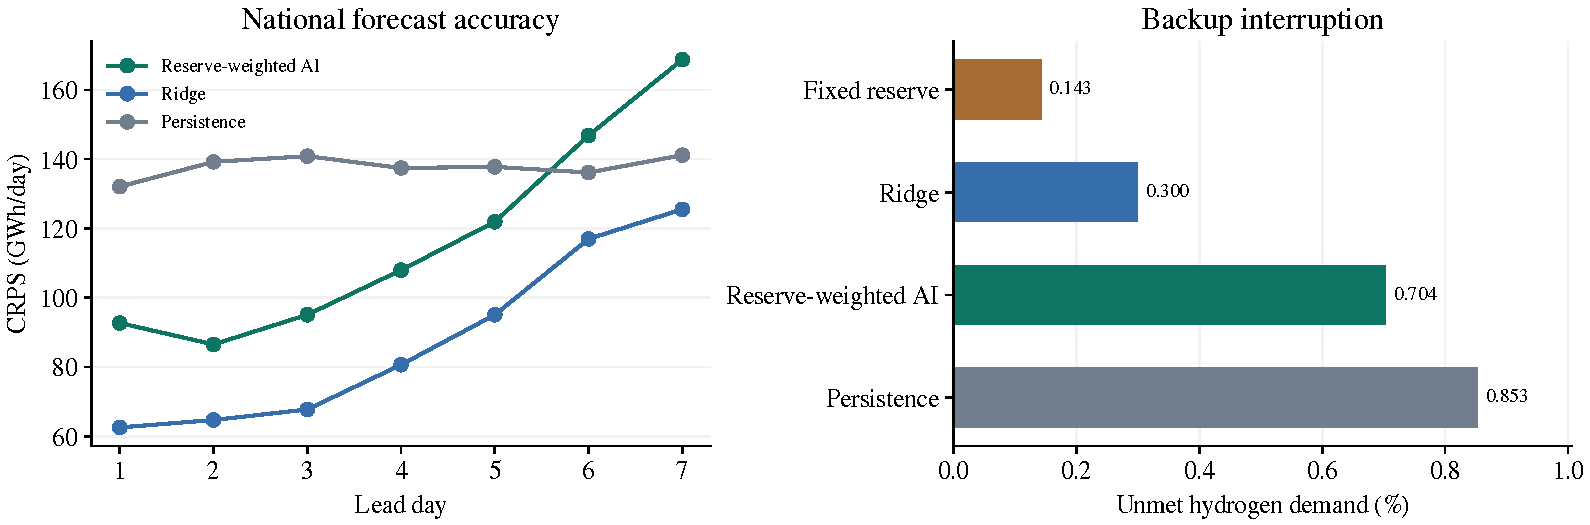
\includegraphics[width=\linewidth]{figures/decision-comparison.pdf}
\caption{Held-out generation forecast skill and delivery reliability. The left panel shows national CRPS by lead. The right panel shows unmet demand during the modeled backup interruption. The fixed-reserve rule has an operational result and uses no separate national forecast.}
\label{fig:comparison}
\end{figure}

\begin{figure}[H]
\centering
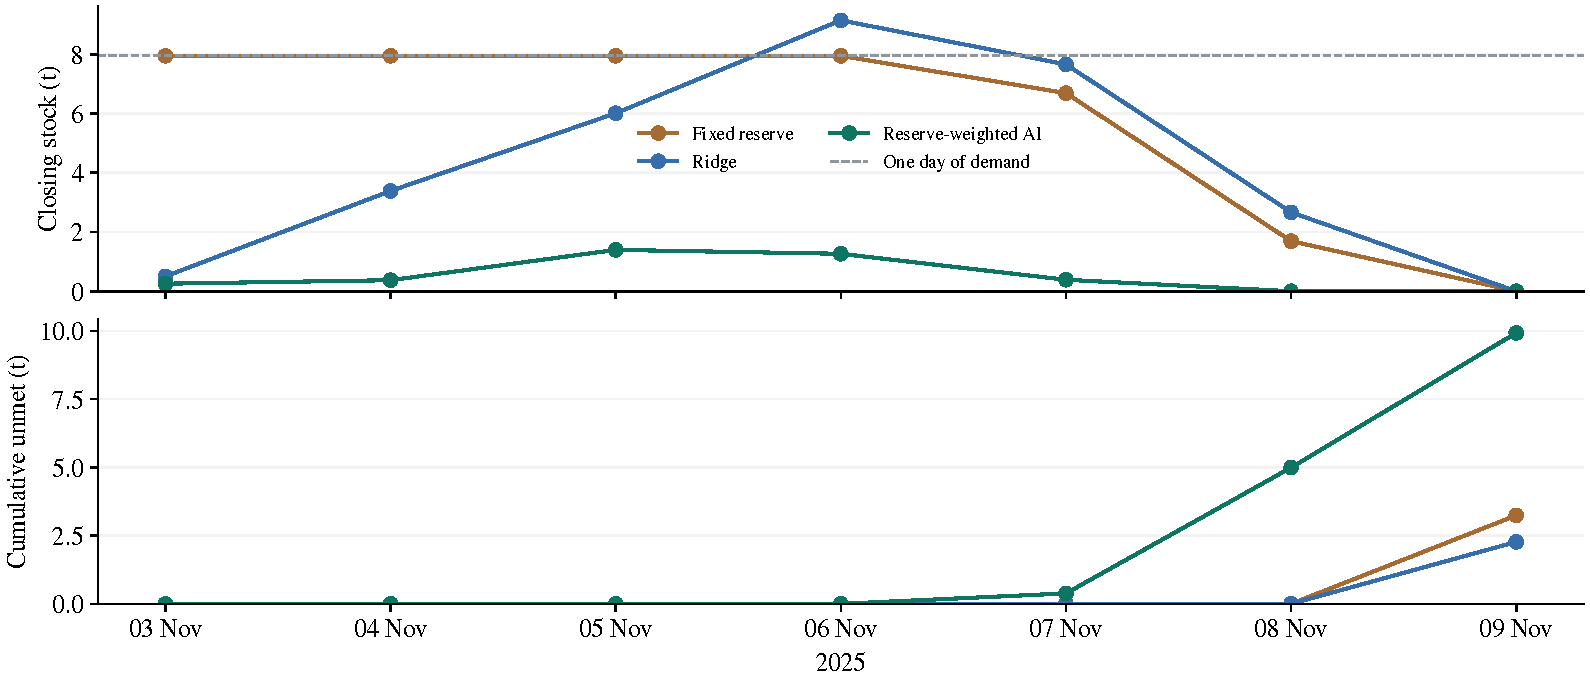
\includegraphics[width=\linewidth]{figures/reserve-episode.pdf}
\caption{Closing inventory and cumulative missed hydrogen deliveries in the focal policy's worst seven-day window under the backup interruption. All policies used the same realized German generation. The dashed line is one day of portfolio demand.}
\label{fig:episode}
\end{figure}

\section{Reproducing the experiment}
The \studyrepo\ hosts code, data retrieval, and fit settings. Use Python 3.12. The following commands reproduce the input extracts, forecast and dispatch results, and exhibits from the repository root.
\begin{verbatim}
python -m pip install -r germany/requirements.txt
python -m germany.data all
python -m germany.run
python -m unittest discover -s tests -v
make -C germany/paper figures PYTHON=python
make -C germany/paper
\end{verbatim}
The \href{\GitHubURL/blob/germany-ai-operations/germany/study.toml}{study configuration} records capacities, dates, and the random seed. The \href{\GitHubURL/blob/germany-ai-operations/germany/report/run_manifest.json}{run manifest} records input checksums and package versions. The \href{\GitHubURL/blob/germany-ai-operations/germany/report/forecast_scores.csv}{forecast metrics} are by lead. The \href{\GitHubURL/blob/germany-ai-operations/germany/report/operations_summary.csv}{operations summary} records each policy and backup case. Detailed replay outputs include per-zone import orders made at issue time, reserve targets, realized production, matched transfers, and opening and closing inventory. The manuscript uses the existing experiment outputs and describes the regional assumptions directly.
